\documentclass[pdf]{beamer}
\usepackage{multicol}
\mode<presentation>{}
\usetheme{Warsaw}
\usepackage{subcaption}
\usepackage{framed}

%\usepackage{listings}

\title{DRL para controle de um levitador magnético}
\author{Gabriel Evangelista}
\begin{document}
\maketitle
\begin{frame}{Ponto de Partida}
	\begin{figure}
	\begin{subfigure}[t]{\textwidth}
		\centering
		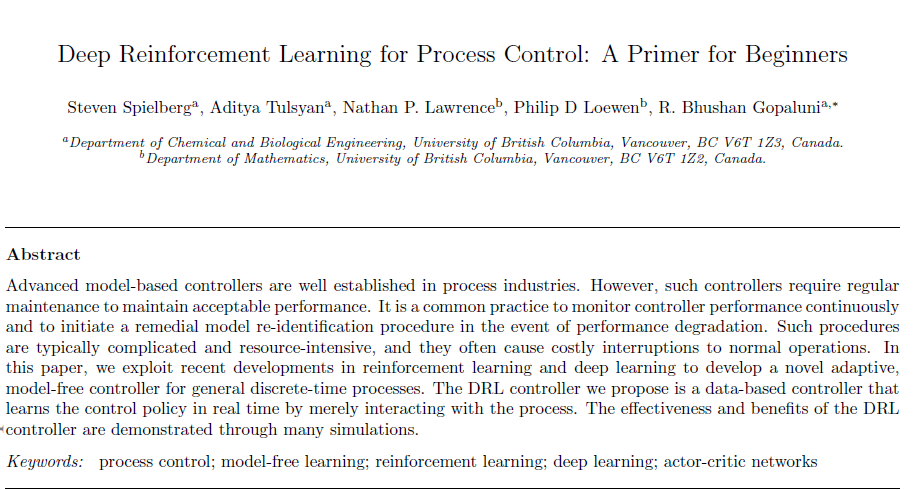
\includegraphics[scale=.5]{img/artigo_inicial.png}
	\end{subfigure}\
	\begin{subfigure}[t]{\textwidth}
		\centering
		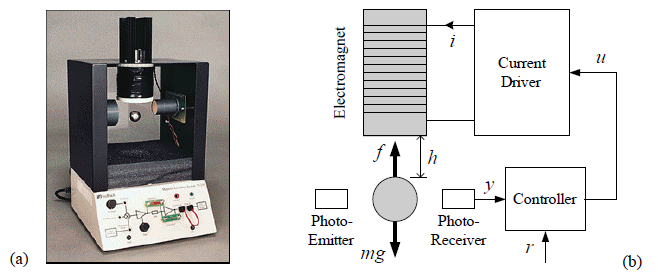
\includegraphics[scale=0.6]{img/planta_kit.png}
	\end{subfigure}
\end{figure}
\end{frame}

\begin{frame}{Reinforcement Learning}
\begin{columns}
	\column{.5\linewidth}
\begin{figure}
	\begin{subfigure}[t]{\textwidth}
		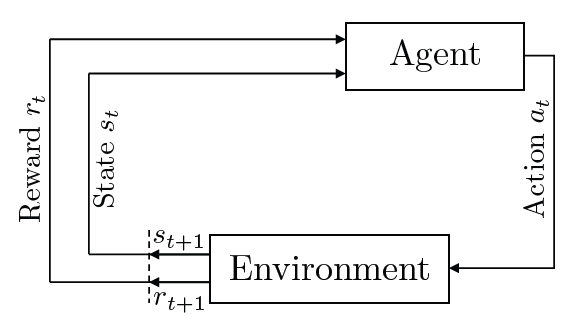
\includegraphics[scale=.5]{img/esquema_rl.png}
	\end{subfigure}

\end{figure}
	\column{.5\linewidth}
	$$ 
	R_t = \sum_{i=t}^{T}{\gamma^{(i-t)}r(s_i, a_i)} 
	$$
	
	$$
	J = \mathbb{E}_{s_i, a_i \sim \pi}[R_1]
	$$
	
	Política: $\pi$ (ou $\mu$ quando determinística).

\end{columns}	
	Equação de Bellman:
	
	$$
	 Q^\mu(s_t, a_t) =  \mathbb{E}_{r_t, s_{t+1}\sim E}[r(s_t, a_t) + \gamma Q^\mu(s_{t+1}, \mu(s_{t+1}))]
	 $$
	
	Onde, usualmente $\mu = argmax_aQ(s_t, a_t)$
	
	Ideia chave: construir um estimador para Q, com parâmetros $\theta$
	
	A perda é dada por:
	
	$$ 
	L(\theta^Q) = \mathbb{E} [(r + \gamma argmax_aQ(s_{t+1}, a_{t+1})|\theta -  Q(s_{t}, a_{t})|\theta )^2] 
	$$	
	

\end{frame}

\begin{frame}{DQN}
\begin{subfigure}[t]{\textwidth}
	\centering
	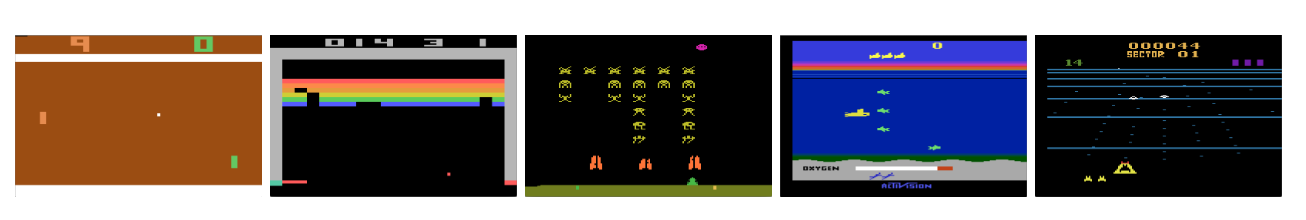
\includegraphics[scale=0.5]{img/atari.png}
\end{subfigure}
Inovações principais:
\begin{itemize}
	\item Target network: 
	$$ 	L(\theta^Q) = \mathbb{E} [(r + \gamma argmax_aQ_{tgt}(s_{t+1}, a_{t+1})|\theta -  Q(s_{t}, a_{t})|\theta )^2]  $$
	\item Memory Buffer: Armazenamento e amostragem de transições. Amostra vai ser mais descorrelacionada e promove um aprendizado melhor do que o as amostras consecutivas.
\end{itemize}

\end{frame}


\begin{frame}{DDPG}
	\begin{itemize}
		\item Usa as técnicas do DQN para implementar a atualização da rede Q
		\item Atualização contínua com uma média: $ \theta_{tgt} \leftarrow \tau\theta + (1 - \tau)\theta_{tgt}$ com $\tau << 1$
		\item Emprega a normalização dos valores
		\item  Ator crítico: Uma rede para gerar as ações e outra para realizar a estimativa do Q
		\item Aprendizado pelo gradiente descendente de J a partir de valores de Q para atualizar $\pi$. 
%		$$
%		\nabla_{\theta^\mu} \approx \mathbb{E}[\nabla_aQ(s,a|\theta^Q)|_{s_t, a=\mu(s_t)}\nabla{\theta^\mu}\mu(s|\theta^\mu)|s_t]
%		$$

		\item \textbf{Ações contínuas!}

	\end{itemize}
\end{frame}

\begin{frame}{DRL Controller}
	
	\begin{subfigure}[t]{\textwidth}
		\centering
		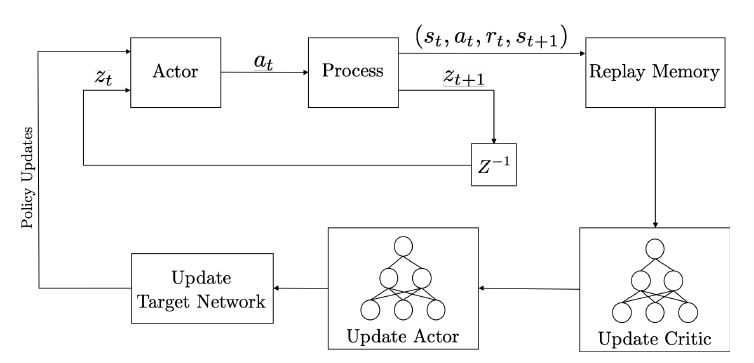
\includegraphics[scale=0.5]{img/DRL_controller.png}
	\end{subfigure}
	\begin{itemize}
		\item Baseado no DDPG
		\item Utiliza uma técnica de \textit{gradient clip}
		\item Adiciona a variável de referência no algoritmo
		\item Relaciona as abordagens dos problemas:
		
		\subitem $ a_t = f^{-1}(u_t)$
		
		\subitem $ s_t = < y_t, y_{t-1}, ... y_{t-d}, a_t, a_{t-1}, ..., a_{t-d}, (y_t - y_{sp}) >$ 
		
		\subitem $ r_t = -| y_t - y_{sp}| $, ou outra que se adapte ao problema, em função de $ y_t  $ e $ y_{sp} $.
		
		
	\end{itemize}
\end{frame}


\begin{frame}{A planta estudada}
	\begin{columns}
		\column{.5\linewidth}
		\begin{subfigure}[t]{\textwidth}
			\centering
			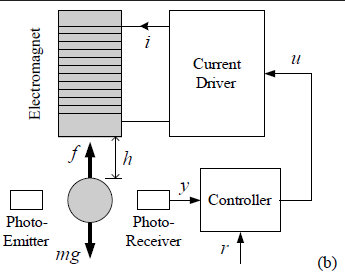
\includegraphics[scale=0.75]{img/esquema_planta.png}
		\end{subfigure}
		\column{.5\linewidth}
		
		 $$ f = K \frac{i^2}{h^2}$$
		 $$
		 m\frac{d^2h}{dt^2} = mg - K\frac{i^2}{h^2} 
		 $$
		 $$ y = \gamma h + y_0, y \in (-2V, 2V) $$
		 $$ i = \rho u + i_0, u \in (-3V, 5V) $$		 
		 $$\boxed{
		 \frac{d^2 y}{dt^2} = \gamma g - \frac{K(\rho u + i_0)^2\gamma^3}{m(y - y_0)^2}}
		 $$
		 
		 $$\dot{x_1} = x_2 $$		 
		 $$ \dot{x_2} =  \gamma g - \frac{K(\rho u + i_0)^2\gamma^3}{m(y - y_0)^2} $$
	\end{columns}
		 
%No espaço de estados, com 

\end{frame}

\begin{frame}{Resultado na Planta Proposta}
	

		\begin{columns}
		\column{.4\linewidth}

			$$s_t = < (y_t - ref), y_t, dy_t, u_t >$$			
			$$	u_t = u_{t-1} + a_t $$			
			$$ ref \rightarrow Const$$
			$$ ref \in (-0.5, 0.5), run-by-run $$
			
			
		\boxed{$$ rwd = -\exp(-e^2/0.05) $$}
		$ \\\\ $
			
			
		Erros quadráticos médios (0.0133):
		
		 0.0256,
		 
		 0.0090, 
		 
		 0.0037, 
		 
		 0.0053, 
		 
		 0.0103,
		 
		 0.0256
		 
		  

		\column{.6\linewidth}
		\begin{subfigure}[t]{\textwidth}
			\centering
			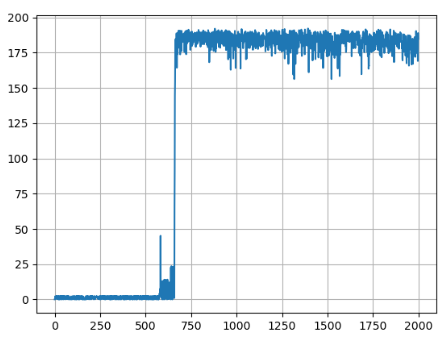
\includegraphics[scale=0.6]{img/aprendizado_exp005.png}
		\end{subfigure}
		\begin{subfigure}[t]{\textwidth}
			\centering
			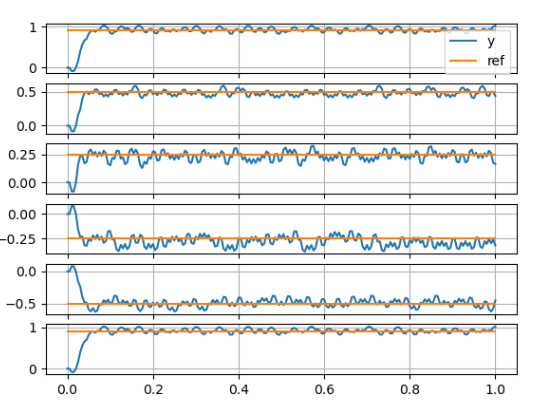
\includegraphics[scale=0.6]{img/resultado_exp005.png}
		\end{subfigure}
	\end{columns}
	
\end{frame}
%
%
%\begin{frame}{Resultado na Planta Proposta}
%	\begin{columns}
%		\column{.4\linewidth}
%		\boxed{$$ rwd =  \begin{cases}
%				1, |e| < 0.025 \\
%				0.5\exp{(-e^2/0.5)} 
%			\end{cases}   
%		)$$}
%		$ \\ $
%		
%		
%		Erros quadráticos médios (0.0142):
%		
%	0.0250, 
%	
%	0.0089, 
%	
%	0.0043, 
%	
%	0.0071,
%	
%	0.0147, 
%	
%	0.0250 
%		
%		
%		
%		\column{.6\linewidth}
%		\begin{subfigure}[t]{\textwidth}
%			\centering
%			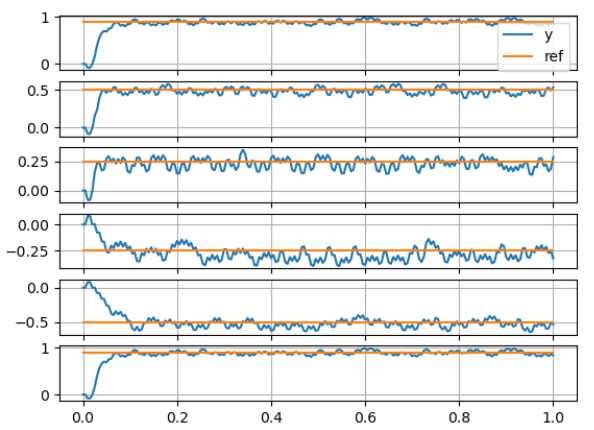
\includegraphics[scale=0.6]{img/resultado_discont.png}
%		\end{subfigure}
%	\end{columns}
%	
%\end{frame}


\begin{frame}{Resultado na Planta Proposta}
	\begin{columns}
		\column{.4\linewidth}
		\boxed{$$ rwd = -\exp(-e^2/0.05) 
			\\
			-0.75\Delta u^2$$}
		$ \\\\ $
		
		
		Erros quadráticos médios (0.0152):
		
		0.0308, 
		
		0.0095,
		
		0.0042, 
		
		0.0044, 
		
		0.0111,
		
		0.0308

		
		\column{.6\linewidth}
		$\\$
		
		\begin{subfigure}[t]{\textwidth}
			\centering
			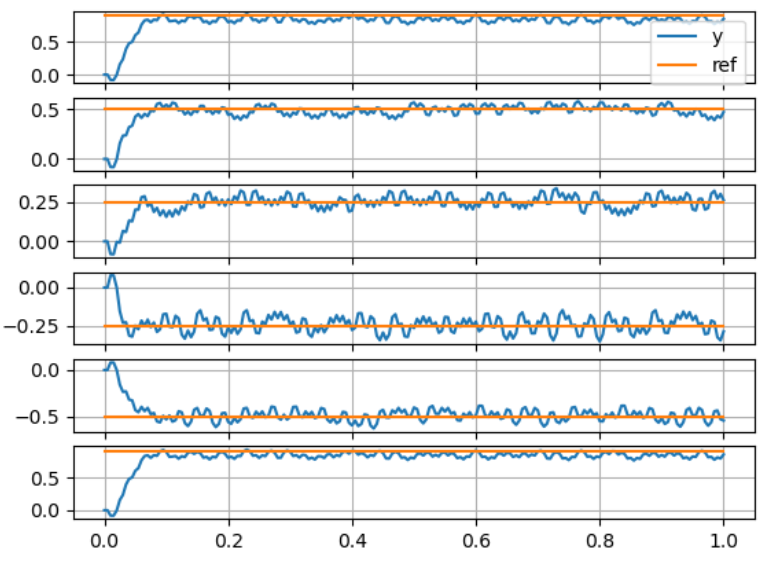
\includegraphics[scale=0.45]{img/resultado_opt.png}
		\end{subfigure}
	\end{columns}
	
\end{frame}


\begin{frame}{Reprodução do Resultado Original}
	$$ G(z) = \frac{0.05z^{-1}}{1 - 0.6z^{-1}}$$
\begin{columns}
	\column{.5\linewidth}
		\begin{subfigure}[t]{\textwidth}
			\centering
			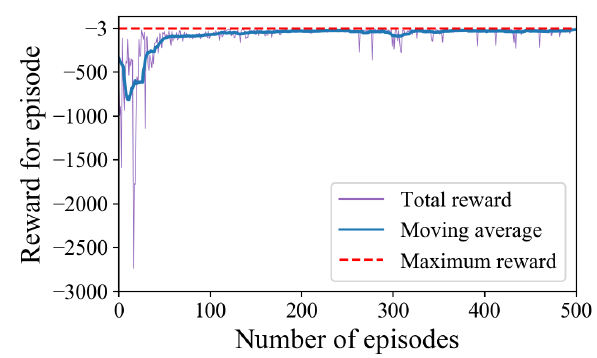
\includegraphics[scale=0.5]{img/result_original_paper_aprendizado.png}
		\end{subfigure}
		\begin{subfigure}[t]{\textwidth}
			\centering
			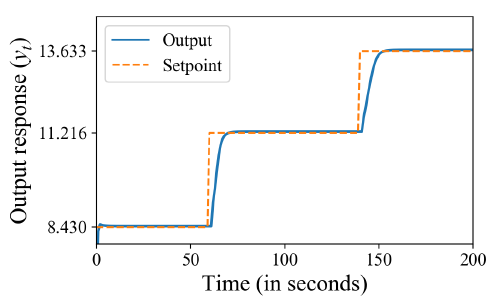
\includegraphics[scale=0.5]{img/result_original_paper_steps.png}
		\end{subfigure}
	\column{.5\linewidth}
		\begin{subfigure}[t]{\textwidth}
			\centering
			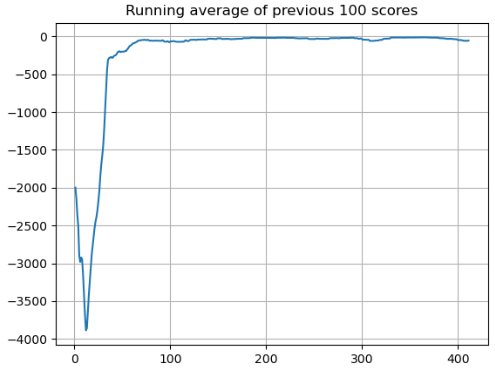
\includegraphics[scale=0.45]{img/result_original_aprendizado.png}
		\end{subfigure}
		\begin{subfigure}[t]{\textwidth}
			\centering
			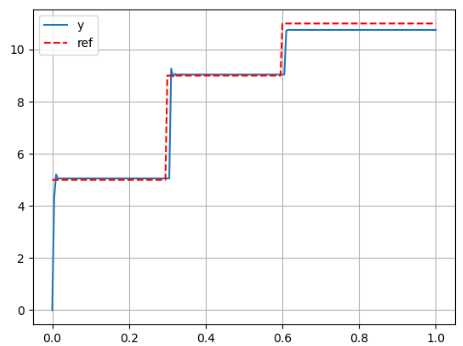
\includegraphics[scale=0.45]{img/result_original_mult_step.png}
		\end{subfigure}
%		\begin{subfigure}[t]{\textwidth}
%			\centering
%			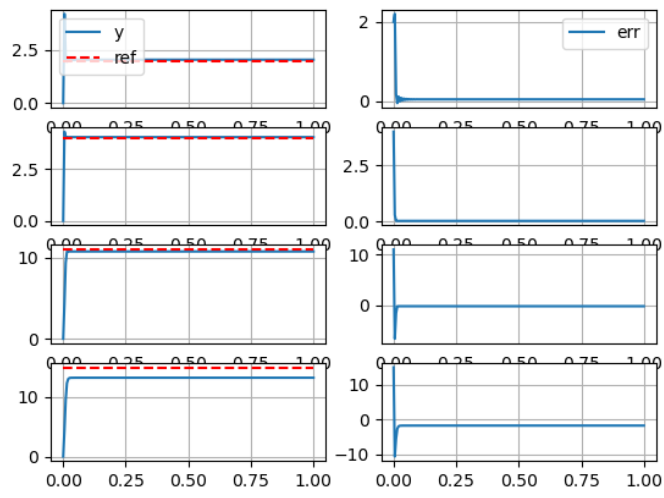
\includegraphics[scale=0.5]{img/result_original_diferent_steps.png}
%		\end{subfigure}
\end{columns}
	
\end{frame}


\begin{frame}{Conclusão}
	\begin{itemize}
		\item As funções de recompensa apresentadas no artigo original não tratam bem problemas instáveis. A instabilidade gera o "morte prematura" do agente caso não hajam recompensas positivas para incrementos do número de passos dados.
		
		\item Apesar da solução funcionar bem nas plantas apresentadas no artigo original, houve dificuldade do emprego da técnica em uma planta instável.

	\end{itemize}
	
\end{frame}

\end{document}
